%========================================================================================
% TU Dortmund, Informatik Lehrstuhl VII
%========================================================================================

\chapter{Einleitung}
\label{Einleitung}

\section{Motivation und Hintergrund}
\label{Motivation_und_Hintergrund}
%
Das Höchstspannungsnetz, welches sich über Deutschland erstreckt ist riesig und besteht aus tausenden von Strommasten und Verbindungen. Da ist sehr vom Nutzen eine Karte zu haben, die einige Verbindungen und Orte verschiebt um eine weitaus bessere und übersichtlichere Darstellung zu erhalten. Das ist genau die Methode einer MetroMap, den Verlust genauer Daten um sicherzustellen, dass die wichtigen Verbindungen und Standorte schnell und sicher erkannt werden.\\

Die Erstellung einer MetroMap von Netzen, findet bisher fast ausschließlich manuell statt. Das heißt, die dafür Zuständigen drehen und verschieben die Knoten auf der eigentlichen Karte, bis es eine, für sie schöne, Darstellung des Netzes wird. Es gibt bereits einige sehr gute Lösungsansätze für eine automatische Anfertigung einer MetroMap. Diese beschränken sich jedoch auf die normalen Bus- und Bahnnetzen. Die Modellierung des Höchstspannungsnetzes und dessen Darstellung als MetroMap erfordert eine Anpassung der momentanen Ansätze. Demnach wird es in dieser Arbeit gezeigt, wie es möglich ist aus einem Teil eines Höchstspannungsnetzes eine MetroMap ähnliche Darstellung zu erhalten, die die Eigenheiten, des Höchstspannungsnetzes berücksichtigt.




\section{Aufbau der Arbeit}
\label{Aufbau_der_Arbeit}
%
In dieser Arbeit geht es darum, die Methoden einer MetroMap für Bus- und Bahnverbindungen zu nutzen, um eine angepasste MetroMap für das deutsche Höchstspannungsnetz zu erhalten. Dafür wird der Sachverhalt eines Höchstspannungsnetzes kurz erläutert. Anschließend werden die benötigten Sachen im Bezug des Graphen definiert, die gebraucht werden um aus dem Höchstspannungsnetz einen repräsentierenden Graphen zu erhalten. \\

Anschließend wird aus einem Teil des Höchstspannungsnetzes ein Graph gewonnen, der auch die Eigenheiten des Netzes modelliert. Dies sind besonders die Leiterseile. Das wird auch der größte und wichtigste Unterschied im Vergleich zu einer normalen MetroMap sein, welcher sich doch deutlich von einer MetroMap eines Bus- oder Bahnnetzes unterscheidet. Auf diesen Graphen ist es nun möglich einen in Kapitel 3 vorgestellten Algorithmus zur Bildung einer MetroMap konformen Darstellung anzuwenden. Dieser Algorithmus wird ein sogenannter Spring-Embedder sein. Dieser beruht auf ein physikalisches Verfahren, welches auf den Graphen modelliert wird, um ein deutlich schöneres Layout zu erhalten. Dieser Algorithmus wurde benutzt, da er sehr leicht erweiterbar ist und sich gut für Anpassungen eignet.\\

Dieser Algorithmus wird nun auf den gewonnen Graphen aus Kapitel 2, welcher den Teil des Höchstspannungsnetzes modelliert, angewendet. Darauf wird besonders auf die Probleme, die die Eigenheiten des Höchstspannungsnetzes mit sich bringen, eingegangen und versucht diese zu lösen. Ebenso werden weitere Erweiterungsmöglichkeiten erläutert und erklärt. Letztendlich werden die erarbeiteten Lösungsansätze evaluiert und beurteilt.
\begin{figure}[t]
	\centering
	{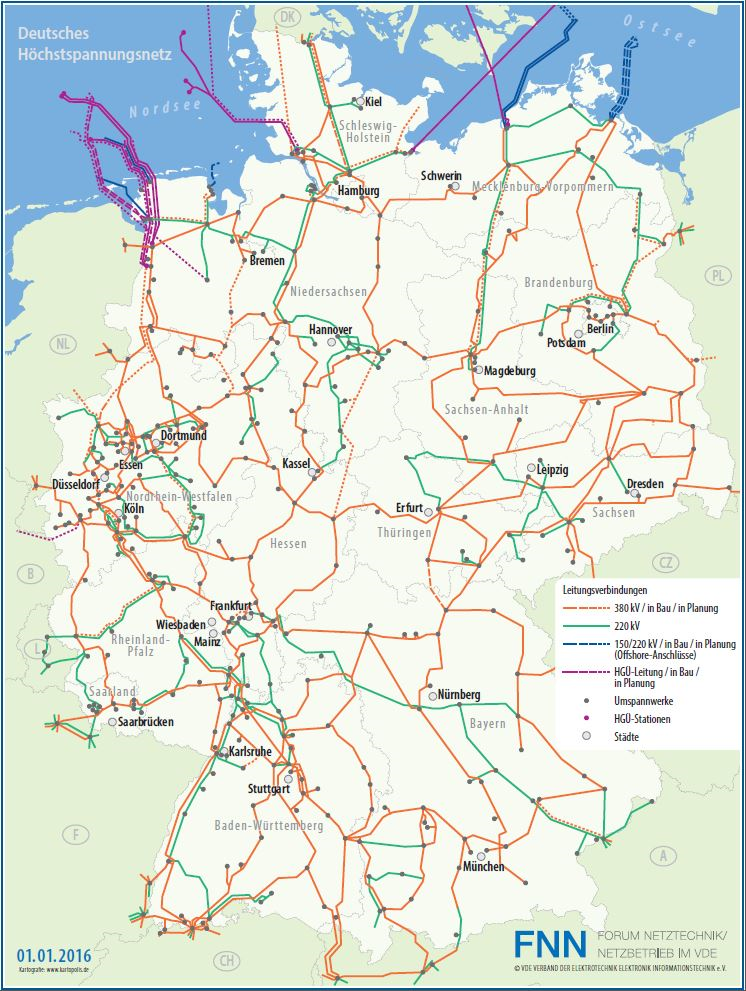
\includegraphics[scale=0.5]{bilder/hochstspannungsnetz}\label{fig_hochstspannungsnetz}
	}\\
	\caption[Karte des deutschen Höchstspannungsnetzes]{Karte des deutschen Höchstspannungsnetzes}
	\label{fig_hochstspannungsnetz2}
\end{figure}

\begin{figure}[t]
	\centering
	{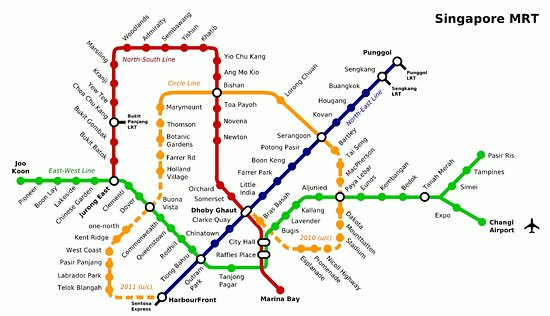
\includegraphics[scale=0.5]{bilder/metromapsinga}\label{fig_metromapsinga}
	}\\
	\caption[MetroMap der Bahnverbindungen in Singapur]{MetroMap der Bahnverbindungen in Singapur}
	\label{fig_metromapsinga2}
\end{figure}